\documentclass{article}
\usepackage{amsmath}
\usepackage{amssymb}
\usepackage{graphicx}
\usepackage{hyperref}
\usepackage[version=4]{mhchem}


\begin{document}
\section*{Problem}
As shown in the figure, \(A B C D\) is a trapezoid. Half circle \(O\) is inscribed into \(A B C D\). Find \(A B\) if \(B C=2\) and \(D A=3\).\\
\centering
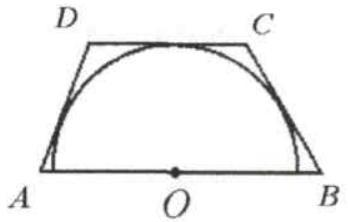
\includegraphics[width=\textwidth]{images/156(1).jpg}

\section*{Solution}
5.
Connect \(O C, O D\).\\
Let the radius of the semicircle be \(r\).\\
In \(\triangle A O D\), the height on \(A O\) and the height on \(A D\) have the same value of \(r\). So \(A O=A D\).\\
Similarly we get \(B O=B C\).\\
\centering
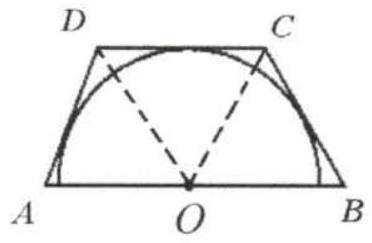
\includegraphics[width=\textwidth]{images/160(1).jpg}

Thus \(A B=B C+D A=5\).

\end{document}
